\makeatletter
\def\input@path{{../../}}
\makeatother
\documentclass[../../main.tex]{subfiles}

\graphicspath{
	{../../img/}
	{../img/}
	{img/}
}

\begin{document}
\section{Интегрируемая ФКП и основные свойства интеграла}
В комплексной плоскости рассмотрим некоторый ориентированный путь,
заданный параметрами
\begin{equation}
    \label{lec30_2:1}
    l:
    \begin{cases}
        z = x(t) + iy(t),\\
        x, y \in \R,\\
        \alpha \leq t \leq \beta,
    \end{cases}
\end{equation}
движение по которому в соответствии с использованными параметрами 
проходит от точки $z(\alpha) = x(\alpha) + 
iy(\alpha)$ до точки 
$z(\beta) = x(\beta) + iy(\beta).$

В соответствии с ориентацией произведём разбиение кривой $l=
\overbowright{z_\alpha z_\beta}$ 
на $n$ произвольных частей последовательными точками
$A = z_0,\ z_1,\ z_2, \ldots,\ z_{n-1},\ z_n = B$ на дуги
$l_k = \overbowright{z_{k-1}z_k},\ k = \overline{1, n}$.

\begin{center}
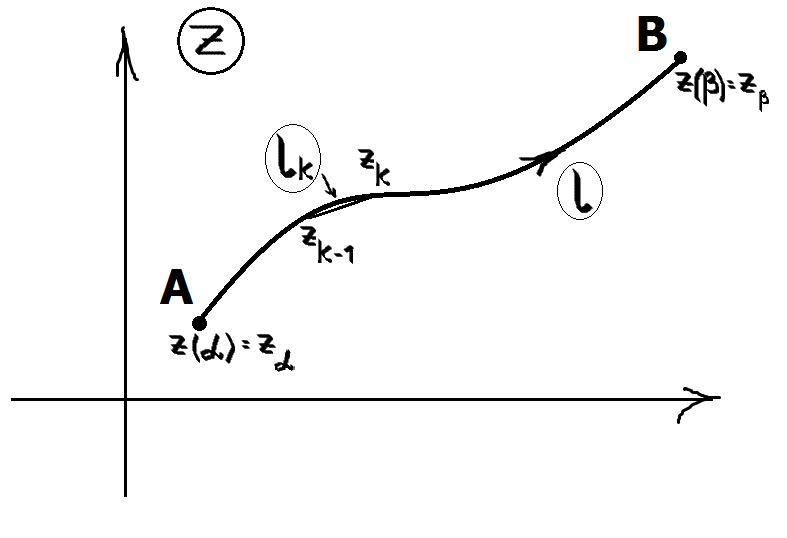
\includegraphics[height=0.4\textwidth]{lec30_9.png}
\end{center}

Пусть $d = \max |\Delta z_k|,\ \text{где } \Delta z_k = z_k - z_{k-1},\ 
k = \overline{1, n}.$ Тогда $d = \diam P$~--- диаметр нашего разбиения $P$
точками $z_i,\ i = \overline{0, n}.$ На каждой дуге разбиения $l_k$ 
выберем отмеченные точки $M_k \in l_k,\ k = \overline{1, n}.$ 
Если на исходной кривой определена функция $w = f(z), $ то в 
соответствии с использованным разбиением $P$ с множеством отмеченных точек
${S = \{M_k\}_{k=1}^n}$ можно составить интегральную сумму
\begin{equation}
    \label{lec30_2:2}
    \sigma = \sigma\left(f, \{P, S\}\right) =
    \sum_{k=1}^{n}{f\left(M_k\right)\Delta z_k}.
\end{equation}
Функция $f(z),\ z \in l$ называется \emph{интегрируемой на $l$}, 
если
\begin{equation}
    \label{lec30_2:3}
    \exists\ I \in \C \quad \forall \eps > 0 \quad \exists \delta = 
    \delta_\eps > 0 \quad
    \forall \{P, Q\},\ d = \diam P \leq \delta \implies
    |\sigma - I| \leq \eps.
\end{equation}
Здесь число $I \in \C$ будем называть \emph{значением интеграла ФКП
$f(z)$ по $l$} и обозначать 
\begin{equation}
    \label{lec30_2:4}
    I = \int\limits_l{f(z) dz} \stackrel{\eqref{lec30_2:2}}{=}
    \lim_{d \to 0}\sigma = \lim_{d \to 0}{\sum_{k=1}^n{
    f\left(M_k\right)\Delta z_k}}.
\end{equation}
Определение интеграла ФКП соответствует определению КрИ-2 для
действительных функций.

Пусть $f(z) = c_0 = const \in \C$. Тогда
\[\sigma \stackrel{\eqref{lec30_2:2}}{=} \sum\limits_{k=1}^n{c_0\Delta z_k} = 
c_0\left(-z_0 + z_1 - z_1 + z_2 - \ldots - z_{n-1} + z_n\right) = 
c_0\left(z_n - z_0\right) = c_0\left(z_\beta - z_\alpha\right).\]

В частности, если $c_0 = 1,$ то
$\displaystyle\int\limits_{\tiny \overbow{z(\alpha)z(\beta)}}{dz} = 
z(\beta) - z(\alpha).$
Если же $c_0 = 0, $ то
$\displaystyle\int\limits_{\tiny\overbow{z_\alpha z_\beta}}{0\;dz} = 0$.

Для вычисления интеграла ФКП через КрИ-2 от действительной функции 
рассмотрим функции от двух переменных
\begin{equation*}
 \begin{cases}
  u = u\left(x, y\right) = \Re f(z),\\
  v = v\left(x, y\right) = \Im f(z).
 \end{cases}
\end{equation*}
Используем разбиение точками $P = \{z_k\}$, где $z_k = x(t_k) + y(t_k)$, 
причем $\{t_k\}_{k=0}^n $~--- соответствующие точки разбиения 
$\left[\alpha,\beta\right]$. Множество отмеченных точек
$S = \{M_k\} = \{(x(\tau_k), y(\tau_k))\}$. Тогда рассматриваемую интегральную 
сумму 
$\eqref{lec30_2:2}$ запишем в виде
\[\sigma = \sum\limits_{k=1}^n{\left(u(x(\tau_k), y(\tau_k))
+ iv(x(\tau_k), y(\tau_k))\right)\left(\Delta x_k + 
i\Delta y_k\right)},\] 
где
\begin{gather*}
\Delta x_k = x(t_k) - x(t_{k-1}),\\
\Delta y_k = y(t_k) - y(t_{k-1}).
\end{gather*}
Отделяя действительную и мнимую части, имеем
\[
\sigma = \sum_{k=1}^n{(u(x(\tau_k), y(\tau_k))\Delta x_k -
v(x(\tau_k), y(\tau_k))\Delta y_k)} + 
i\sum_{k=1}^n{(u(x(\tau_k), y(\tau_k))\Delta y_k + 
v(x(\tau_k), y(\tau_k))\Delta x_k)}.
\]
Переходя к пределу 
$d = \underset{1 \leq k \leq n}{\max}|\Delta z_k| = 
\underset{1 \leq k \leq n}{\max}\sqrt{\Delta x_k^2 + \Delta y_k^2}
\longrightarrow 0 \implies
\begin{cases}
    \Delta x_k \longrightarrow 0,\\
    \Delta y_k \longrightarrow 0,
\end{cases}$ \hspace{-1em}
получаем в силу определения КрИ-2 для действительных Ф2П:
\[
\sigma \underset{d \to 0}{\longrightarrow} \int\limits_l{
udx - vdy} + i\int\limits_l{udy + vdx},
\]
т.~е.
\begin{equation}
    \label{lec30_2:5}    
    \int\limits_{l}{f(z)dz} = \int\limits_l{udx - vdy} + 
    i\int\limits_l{udy + vdx}.
\end{equation}
\eqref{lec30_2:5} можно также формально получить следующим образом:
\begin{gather*}
f(z) = u + iv, \quad
dz = dx + idy, \\
\int\limits_l{\left(u+iv\right)\left(dx + idy\right)} = 
\int\limits_l{udx - vdy} + i\int\limits_l{udy + vdx} 
\iff \eqref{lec30_2:5}.
\end{gather*}

В частности, если $l$ имеет параметризацию $\eqref{lec30_2:1},$ то в 
этом случае получаем
\[I = \left[
\begin{array}{c}
     x = x(t)\quad dx = x'(t)dt \\
     y = y(t)\quad dy = y'(t)dt \\
     \alpha \leq t \leq \beta\\
\end{array} 
\right]=\]
\[\stackrel{\eqref{lec30_2:5}}{=}
\int\limits_\alpha^\beta{\left(u(x(t), y(t))x'(t) - 
v(x(t), y(t))y'(t)\right)dt} + i\int\limits_\alpha^\beta{
\left(u(x(t), y(t))y'(t) + v(x(t), y(t))x'(t)\right)dt}.
\]

\begin{iexample}
    Пусть $n \in \Z.$ Рассмотрим интеграл
    \[I_n = \int\limits_{|z-z_0| = R}{\frac{dz}{\left(z-z_0\right)^n}}.\]
    Используя параметризацию этой окружности $
    \begin{cases}
     z=z_0 + R e^{it}, \\
    0 \leq t \leq 2\pi,
    \end{cases}$ \hspace{-1em} имеем
    $dz = iRe^{it}dt$.
    Значит, 
    \[I_n = \int\limits_0^{2\pi}{\frac{iRe^{it}dt}{
    (R e^{it})^n}} = \frac{i}{R^{n-1}}\int\limits_0^{2\pi}{
    e^{(1-n)it}dt}.\]
    Если $n \neq 1, $ то \[I_n = \frac{i}{R^{n-1}}\frac{
    e^{(1-n)it}}{(1-n)i}\bigg|_0^{2\pi} = \frac{
    (e^{2\pi i(1-n)}-1)}{R^{n-1}(1-n)} = 0.\]
    Для $n=1$ имеем \[I_1 = i\int\limits_0^{2\pi}{dt} = 2\pi i.\]
    Таким образом, получаем 
    \begin{equation}
        \label{lec30_2:6}
        \int\limits_{|z-z_0| = R}{\frac{dz}{(z-z_0)^n}} = 
        \begin{cases}
            0,& n \neq 1 \in \Z,\\
            2i\pi,& n = 1.
        \end{cases}
    \end{equation}
\end{iexample}

Из полученной формулы вычисления интеграла ФКП через соответствующие
действительные КрИ-2 на основании основных свойств КрИ-2 получим 
следующие свойства интеграла ФКП:

\begin{enumerate} 
  \item \emph{Зависимость от выбранной ориентации пути.} 
$\displaystyle\int\limits_{\tiny\overbowright{AB}}{f(z)dz} = 
-\int\limits_{\tiny\overbowright{BA}}{
f(z)dz}$.

\item \emph{Линейность.} Если $f$ и $g$ интегрируемы на $l$ в 
комплексной плоскости, то тогда
\[\forall \lambda, \mu \in \C \quad \exists \int\limits_l{\left(
\lambda f + \mu g\right)dz} = \lambda\int\limits_l{f\;dz} + 
\mu\int\limits_l{g\;dz}.\]

\item \emph{Аддитивность.}
Если $l = l_1 \cup l_2,$ причём $l_1$ и $l_2$, во-первых, имеют общие
только граничные точки и, во-вторых, ориентированы так же, как $l$, то
тогда для интегрируемой на $l$ ФКП $f$ имеем:
\[\int\limits_{l_1\cup l_2}{f(z)dz} = 
\int\limits_{l_1}{f(z)dz} + \int\limits_{l_2}{f(z)dz}.\]

\item \emph{Основная оценка интеграла ФКП.}
Если $f(z)$ интегрируема на $l$, то
\[\left|\int\limits_l{f(z)dz}\right| \leq \int\limits_l{
|f(z)||dz|} \text{~--- КрИ-1,}\] где
$|dz| = \sqrt{dx^2 + dy^2} $~---  дифференциал дуги.

Доказательство следует из соответствующей оценки для 
$\eqref{lec30_2:2}$:
\[|\sigma| \stackrel{\eqref{lec30_2:2}}{=} 
\left|\sum\limits_{k=1}^n{f\left(z(t_k)\right)\Delta z_k}\right| \leq 
\sum\limits_{k=1}^n{|f\left(z(t_k)\right)||\Delta z_k|}
\appr{d \to 0} \int\limits_l{|f(z)||dz|}.\]
В частности, из основной оценки, полагая $M = 
\underset{z\in l}{\sup}\,|f(z)|$, получаем
\[\left|\int\limits_l{f(z)dz}\right| \leq \int\limits_l{M|dz|} = 
M\int\limits_l{|dz|} = Ml_0,\] где $l_0 $~--- длина $l.$
\end{enumerate}

\section{Интеграл ФКП от аналитической ФКП}
Напомним, что $f(z)$ считается аналитической в области $D \subset \C, $
если она дифференцируема в каждой точке $D$.
Так как далее будет понятно, что из существования производной первого
порядка ФКП следует существование всех производных высших порядков этой
ФКП, то аналитическая функция будет бесконечное число раз непрерывно 
дифференцируема на $D.$

\begin{thm}[Интегральная теорема Коши]
Если $f(z)$ непрерывно дифференцируема в односвязной области
$D \subset \C,$ то тогда для любого замкнутого кусочно-непрерывного контура 
выполняется
\end{thm}
\begin{equation}
    \label{lec30_2:7}
    \oint\limits_l{f(z)dz} = 0.
\end{equation}
\end{document}  
